\documentclass[english,14pt]{beamer}
\usetheme{EastLansing}
\usecolortheme{spruce}

\usepackage{xcolor}
\usepackage{listings}
\usepackage{courier}
\usepackage{graphicx}
\usepackage{amsmath}
\usepackage{algorithm2e}
\usepackage{multicol}
\usepackage{hyperref}
\usepackage{textcomp}

% http://mirrors.ibiblio.org/CTAN/macros/latex/contrib/datetime2/datetime2.pdf
\usepackage{babel}
\usepackage[useregional]{datetime2}

% https://tex.stackexchange.com/questions/42619/x-mark-to-match-checkmark
\usepackage{pifont}% http://ctan.org/pkg/pifont

%% https://stackoverflow.com/questions/1435837/how-to-remove-footers-of-latex-beamer-templates
%%gets rid of bottom navigation bars
%\setbeamertemplate{footline}[page number]
%
%gets rid of navigation symbols
\setbeamertemplate{navigation symbols}{}


\usefonttheme[onlymath]{serif}

\definecolor{mGreen}{rgb}{0,0.6,0}
\definecolor{mGray}{rgb}{0.5,0.5,0.5}
\definecolor{mPurple}{rgb}{0.8,0,0.82}
\definecolor{backgroundColour}{rgb}{0.95,0.95,0.92}
\definecolor{lightBlue}{rgb}{0.1, 0.1, 0.8}
\definecolor{darkGreen}{rgb}{0, 0.39, 0}

\newcommand\red[1]{{\color{red} #1}}
\newcommand\green[1]{{\color{green} #1}}
\newcommand\blue[1]{{\color{blue} #1}}
\newcommand\darkGreen[1]{{\color{darkGreen} #1}}

\newcommand{\cmark}{\ding{51}}%
\newcommand{\xmark}{\ding{55}}%

\lstdefinestyle{CStyle}{
    backgroundcolor=\color{backgroundColour},   
    commentstyle=\color{mGreen},
    keywordstyle=\color{magenta},
    numberstyle=\tiny\color{mGray},
    stringstyle=\color{mPurple},
    basicstyle=\footnotesize,
    breakatwhitespace=false,         
    breaklines=true,                 
    captionpos=b,                    
    keepspaces=true,                 
    numbers=left,                    
    numbersep=5pt,                  
    showspaces=false,                
    showstringspaces=false,
    showtabs=false,                  
    tabsize=2,
    language=Python
}

\lstdefinestyle{pseudo}{
        basicstyle=\ttfamily\footnotesize,
        keywordstyle=\color{lightBlue},
        morekeywords={BEGIN,END,IF,ELSE,ENDIF,ELSEIF,PRINT,WHILE,RETURN,ENDWHILE,DO,FOR,TO,IN,ENDFOR,BREAK,INPUT,CONDITIONS},
        morecomment=[l]{//},
        commentstyle=\color{mGreen}
}

\lstset{basicstyle=\footnotesize\ttfamily,breaklines=true}
\lstset{framextopmargin=50pt,tabsize=2}

\title{ENGG1003 - Monday Week 10}
\subtitle{Normal distribution: extension and application \\ Fitting straight line to data}%\\ \& computing integrals}
\author{Steve Weller}
\institute{University of Newcastle}
%\date{\today}
\date{10 May 2021}

% following is a bit of a hack, but forces page numbers (technically: frame numbers) to run 1,2,3,... 
% with titlepage counting as frame 1

\addtocounter{framenumber}{1}
\titlepage

\begin{document}

\begin{flushleft}
{\scriptsize Last compiled:~\DTMnow}
\vspace*{-5mm}
\end{flushleft}
\framebreak

%==============================================================

\begin{frame}[fragile]

\frametitle{Lecture overview}
\begin{enumerate}
	\item Normal distribution
		\begin{itemize}
			\item extension of \emph{standard} normal distribution \\ (previous lecture)
			\item application
		\end{itemize}	
	\item[]
	
	\item Fitting straight line to data
	\begin{itemize}
		\item using Python to fit a straight line to data
		\item application
	\end{itemize}	
\end{enumerate}

\end{frame}

%==============================================================

\begin{frame}[fragile]

\frametitle{$1)$ Normal distributions}

Recap from previous lecture\ldots

Standard normal probability density function (PDF):
\[
\boxed{
f(x) = \frac{1}{\sqrt{2\pi}} e^{-\frac{1}{2}x^2}}
\]

\begin{itemize}
	\item \emph{standard} normal distribution is a special case of normal (Gaussian) distribution
	\item corresponds to parameters \red{$\mathbf{0.0}$} and \blue{$\mathbf{1.0}$} in:
\end{itemize}

{\small
	\texttt{x = np.random.normal(\textbf{\red{0.0}}, \textbf{\blue{1.0}}, size=100000)}
}

\end{frame}

%==============================================================

\begin{frame}[fragile]

\frametitle{Normalized histogram (area $1$), 100 bins}

\begin{figure}[ht]
	\centering
	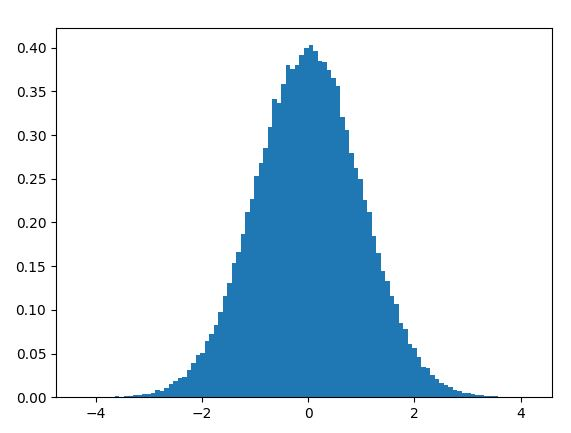
\includegraphics[width=0.7\textwidth]{figures/hist100BinsDensity}
\end{figure}

\vspace*{-5mm}

\begin{itemize}
	\item same histogram, except total area of rectangles is normalized to be $1$
\end{itemize}

\end{frame}


%==============================================================

\begin{frame}[fragile]

\frametitle{Normalized histogram with PDF}

\begin{figure}[ht]
	\centering
	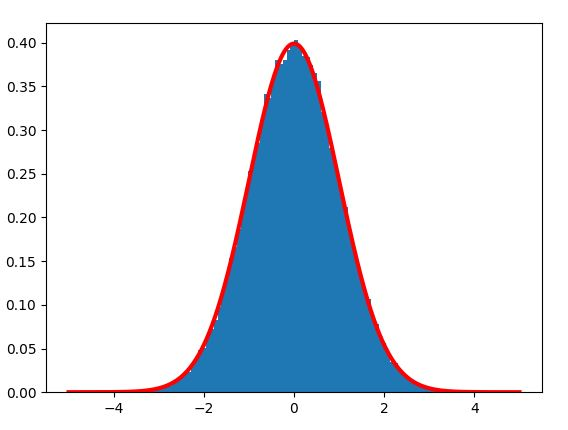
\includegraphics[width=0.7\textwidth]{figures/histWithpdf}
\end{figure}

\vspace*{-5mm}

\begin{itemize}
	\item[] red curve is \red{\emph{probability density function (PDF)}}
\end{itemize}

\end{frame}

%==============================================================

\begin{frame}[fragile]

\frametitle{Probability density functions}

If $X$ is a random number drawn from a distribution with PDF $f(x)$, probability $X$ takes a value in interval $[a,b]$ is
\vspace*{-2mm}
\[
	\boxed{
\mathrm{P}(a \leq X \leq b) = \int_a^b f(x) dx}
\]
\vspace*{-5mm}
\begin{figure}[ht]
	\centering
	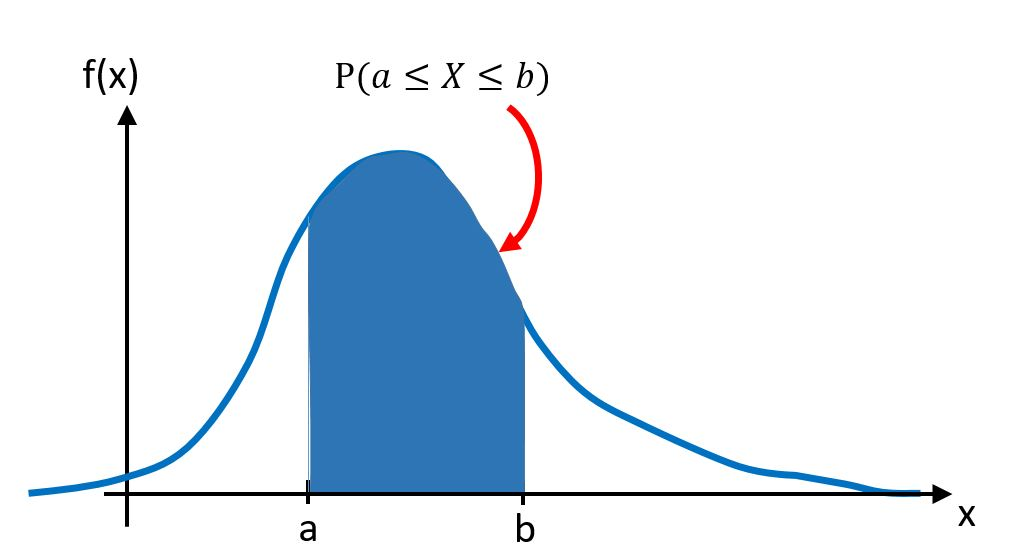
\includegraphics[width=.7\textwidth]{figures/genericPDF}
\end{figure}

\end{frame}

%==============================================================

\begin{frame}[fragile]

\frametitle{Example}

Use trapezoidal method to approximate $\mathrm{P}(1 \leq X \leq 2)$ when $X$ is drawn from standard normal distribution
\[
\mathrm{P}(1 \leq X \leq 2) = \frac{1}{\sqrt{2\pi}} \int_1^2 e^{-x^2/2} dx \approx \mathbf{\red{0.1359}}
\]

\vspace*{-5mm}
\begin{figure}[ht]
	\centering
	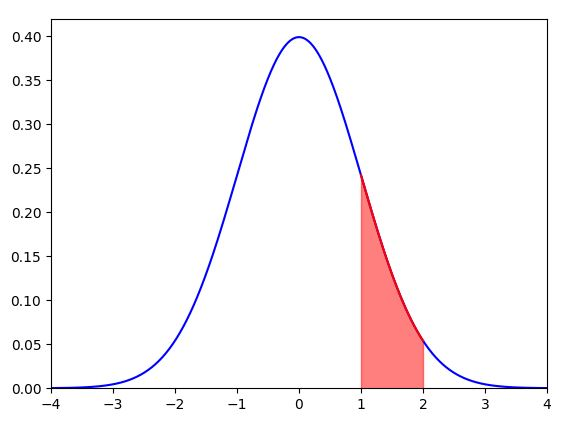
\includegraphics[width=.5\textwidth]{figures/stdnormal_12}
\end{figure}

\end{frame}

%==============================================================

\begin{frame}[fragile]

\frametitle{Extending the standard normal distribution}

\begin{itemize}
	\item standard normal is useful, but inflexible
	\item now \textbf{experimentally observe} impact of first two parameters in \texttt{normal()} function call
\end{itemize}

\boxed{
{\small
	\texttt{x = np.random.normal(\textbf{\red{mean}}, \textbf{\blue{SD}}, size=N)}
}}

\begin{itemize}
	\item impact of \red{mean}
	\begin{itemize}
		\item shifts central (average) value of random numbers
		\item left-right shift of PDF
	\end{itemize}
	
	\item impact of \blue{SD}
	\begin{itemize}
		\item SD is short for ``standard deviation''
		\item controls spread of PDF around central value
	\end{itemize}
	
\end{itemize}

\end{frame}

%==============================================================

\begin{frame}[fragile]

\frametitle{Impact of \emph{mean} parameter}

\begin{figure}[ht]
	\centering
	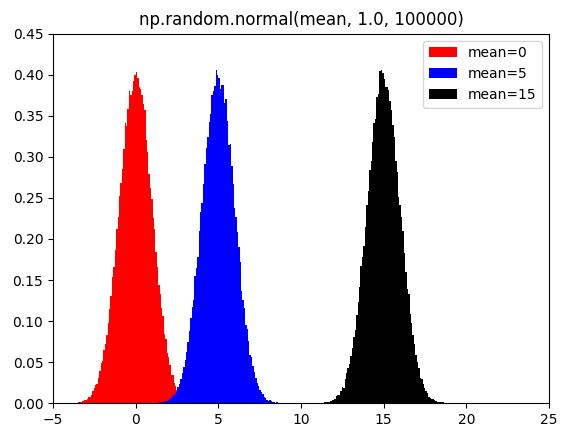
\includegraphics[width=0.65\textwidth]{figures/meanDemoOutput}
\end{figure}

\vspace*{-5mm}

\begin{itemize}
	\item normalized histograms of normal random numbers with mean $=0, 5$ and $15$
\end{itemize}

\end{frame}

%==============================================================

\begin{frame}[fragile]

\frametitle{Python code: impact of mean}

\vspace*{-3mm}

\texttt{meandemo.py}
\vspace*{-1mm}
\begin{lstlisting}[style=CStyle,basicstyle=\scriptsize]
# meandemo
import numpy as np
import matplotlib.pyplot as plt

N = 100000
np.random.seed(1)
x0 = np.random.normal(0.0, 1.0, size=N)
x5 = np.random.normal(5.0, 1.0, size=N)
x15 = np.random.normal(15.0, 1.0, size=N)

plt.hist(x0, 100, density=True, color='r', label='mean=0')
plt.hist(x5, 100, density=True, color='b', label='mean=5')
plt.hist(x15, 100, density=True, color='k', label='mean=15')

plt.title('np.random.normal(mean, 1.0, {})'.format(N))
plt.axis([-5, 25, 0, 0.45])
plt.legend()
plt.show()
\end{lstlisting}

\vspace*{-2mm}

\begin{itemize}
	\item lines 7--13: generate random numbers, plot histograms
\end{itemize}

\end{frame}

%==============================================================

\begin{frame}[fragile]

\frametitle{Impact of \emph{SD} parameter}

\begin{figure}[ht]
	\centering
	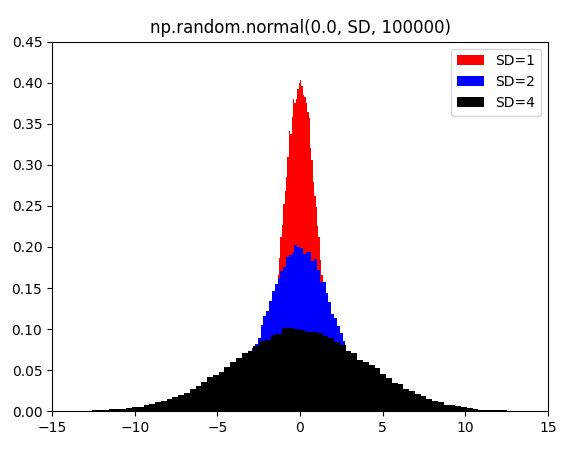
\includegraphics[width=0.65\textwidth]{figures/SDdemoOutput}
\end{figure}

\vspace*{-5mm}

\begin{itemize}
	\item normalized histograms of normal random numbers with SD $=1, 2$ and $4$
\end{itemize}

\end{frame}

%==============================================================

\begin{frame}[fragile]

\frametitle{Python code: impact of SD}

\vspace*{-3mm}

\texttt{SDdemo.py}
\vspace*{-1mm}
\begin{lstlisting}[style=CStyle,basicstyle=\scriptsize]
# SDdemo
import numpy as np
import matplotlib.pyplot as plt

N = 100000
np.random.seed(1)
x0 = np.random.normal(0.0, 1.0, size=N)
x5 = np.random.normal(0.0, 2.0, size=N)
x15 = np.random.normal(0.0, 4.0, size=N)

plt.hist(x0, 100, density=True, color='r', label='SD=1')
plt.hist(x5, 100, density=True, color='b', label='SD=2')
plt.hist(x15, 100, density=True, color='k', label='SD=4')

plt.title('np.random.normal(0.0, SD, {})'.format(N))
plt.axis([-15, 15, 0, 0.45])
plt.legend()
plt.show()
\end{lstlisting}

\vspace*{-2mm}

\begin{itemize}
	\item lines 7--13: generate random numbers, plot histograms
\end{itemize}

\end{frame}

%==============================================================

\begin{frame}[fragile]

\frametitle{Normal PDF}

Mathematical expression for normal PDF:
\[
\boxed{
	f(x) = \frac{1}{\sigma\sqrt{2\pi}} e^{-\frac{1}{2}\left(\frac{x-\mu}{\sigma}\right)^2}}
\]

\begin{itemize}
	\item $\mu = $ mean
	\item $\sigma = $ SD (standard deviation)
	\item what are you expected to do with the normally distributed random numbers in ENGG1003?
	\begin{enumerate}
		\item call \texttt{np.random.normal()} to generate random numbers for specified $\mu$ and $\sigma$
		\item compute probability normally distributed random number $X$ falls in range $[a,b]$ using numerical integration (eg: trapezoidal method)
	\end{enumerate}
\end{itemize}

\end{frame}

%==============================================================

\begin{frame}[fragile]

\frametitle{Standard normal as special case}

Important special case: $\mu=0$ and $\sigma=1$

\[
f(x) = \frac{1}{\sqrt{2\pi}} e^{-\frac{1}{2}x^2}
\]

\vspace*{5mm}

\textbf{Key point:} standard normal distribution has a mean of $0$ and a standard deviation of $1$

\vspace*{5mm}

\boxed{
{\small
	\texttt{x = np.random.normal(\textbf{\red{0.0}}, \textbf{\blue{1.0}}, size=N)}
}}

\vspace*{5mm}

\begin{itemize}
	\item we saw this special case in Thursday week 9 lecture
\end{itemize}

\end{frame}

%==============================================================

\begin{frame}[fragile]

\frametitle{Application: resistor values}

The distribution of resistor values (measured in ohms ($\Omega)$) is observed to follow a normal distribution with mean $\mu=1000$ and SD $\sigma = 30$

\vspace*{5mm}

Write a Python script which:
\begin{enumerate}
	\item plots the PDF of resistance values
	\item uses numerical integration to show that $\approx90$\% of the resistor values fall in the range $[950,1050]~\Omega$
\end{enumerate}

\end{frame}

%==============================================================

\begin{frame}[fragile]

\frametitle{Distribution of resistance values}

\begin{figure}[ht]
	\centering
	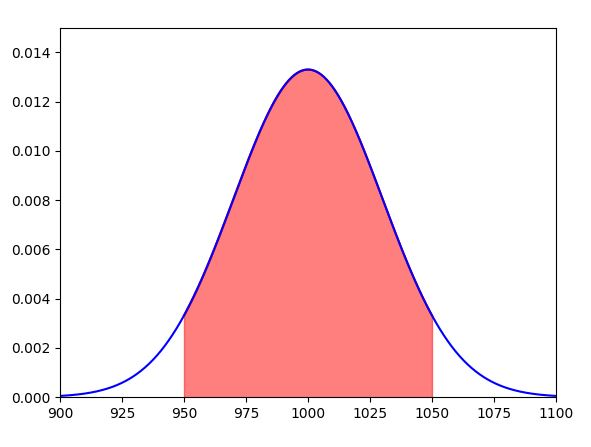
\includegraphics[width=0.65\textwidth]{figures/resistanceoutput}
\end{figure}

\vspace*{-5mm}

\begin{itemize}
	\item blue curve is PDF: mean $=1000$ and SD $=30$
	\item red shaded area ($= 0.9$) shows range $[950,1050]$
\end{itemize}

\end{frame}

%==============================================================

\begin{frame}[fragile]

\frametitle{Python code: resistor values}

\vspace*{-3mm}

\texttt{resistors.py}
\vspace*{-1mm}
\begin{lstlisting}[style=CStyle,basicstyle=\scriptsize]
import numpy as np
import matplotlib.pyplot as plt

def f(x):
    mu = 1000
    sigma = 30
    return 1/(sigma * np.sqrt(2 * np.pi)) * np.exp(-(x - mu)**2 / (2 * sigma**2 ))

def trapezoidal(f, a, b, n):
    h = (b - a) / n
    f_sum = 0
    for i in range(1, n, 1):
        x = a + i * h
        f_sum = f_sum + f(x)
    return h * (0.5 * f(a) + f_sum + 0.5 * f(b))
\end{lstlisting}

\end{frame}

%==============================================================

\begin{frame}[fragile]

\frametitle{Python code: resistor values}

\vspace*{-3mm}

\texttt{resistors.py}---continued
\vspace*{-1mm}
\begin{lstlisting}[style=CStyle,basicstyle=\scriptsize]
a = 950
b = 1050
prob_ab = trapezoidal(f, a, b, 100)
print('Probability resistance in range [{},{}] is: {:.2f} percent'.format(a, b, 100*prob_ab))

x = np.linspace(900, 1100, 1000)
xab = np.linspace(a, b, 100)

plt.plot(xab, f(xab), 'r')
plt.plot(x, f(x), 'b')  # standard normal pdf
plt.fill_between(xab, f(xab), color='r', alpha=0.5)  # alpha=transparency
plt.axis([900, 1100, 0, 0.015])
plt.show()
\end{lstlisting}

\end{frame}

%==============================================================

\begin{frame}[fragile]

\frametitle{$2)$ Fitting straight line to data}

\begin{itemize}
	\item \textbf{Aim:} construct a function that best fits a series of data points
	\begin{itemize}
		\item simplest function is a \emph{straight line}
	\end{itemize}
	\item two common forms of \red{\emph{curve-fitting}} in Engineering applications:
	
	\begin{enumerate}
	\item \red{\emph{interpolation}}
	\begin{itemize}
		\item week 6, Monday lecture
	\end{itemize}
	\item[]
	\item \red{\emph{regression}}
	\begin{itemize}
		\item today's lecture
	\end{itemize}
\end{enumerate}

\end{itemize}
	
\begin{itemize}
	\item we now demonstrate both curve-fitting methods applied to the same dataset
\end{itemize}

\end{frame}

%==============================================================

\begin{frame}[fragile]

\frametitle{Curve-fitting dataset}

\texttt{Week6Monday.py}
\vspace*{-3mm}
\begin{figure}[ht]
	\centering
	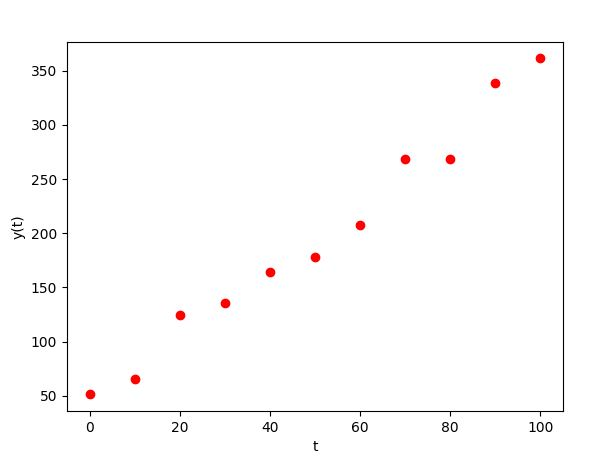
\includegraphics[width=0.6\textwidth]{figures/Week6MonDataset}
\end{figure}
\vspace*{-5mm}
\begin{itemize}
	\item 11 pairs of data points $(t_i,y_i), i = 0,1,2,\ldots,10$
	\item[] {\small $(0,51.29), (10,65.24), (20,124.89), \ldots,(100,361.32)$}
\end{itemize}

\end{frame}

%==============================================================

\begin{frame}[fragile]

\frametitle{Interpolation}

\vspace*{-3mm}
\begin{figure}[ht]
	\centering
	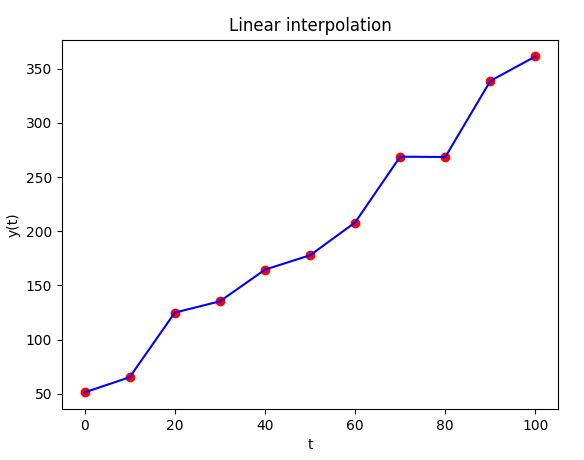
\includegraphics[width=0.8\textwidth]{figures/Week6MonLinearInterp}
\end{figure}

\end{frame}

%==============================================================

\begin{frame}[fragile]

\frametitle{Regression: straight-line fit}

\vspace*{-3mm}
\begin{figure}[ht]
	\centering
	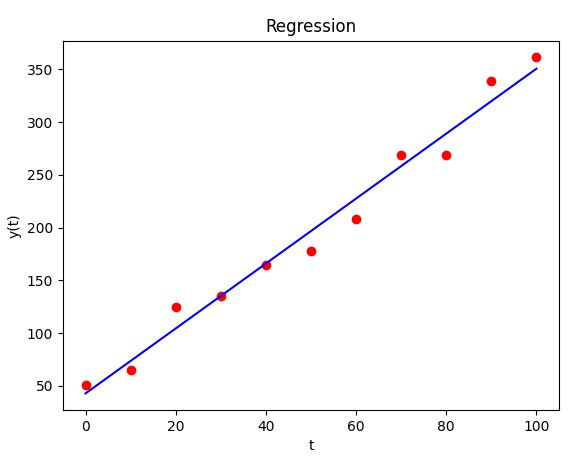
\includegraphics[width=0.8\textwidth]{figures/Week6MonLinearRegression}
\end{figure}

\end{frame}

%==============================================================

\begin{frame}[fragile]

\frametitle{Interpolation vs.\ regression}

\begin{itemize}
	\item \textbf{interpolation:} joining the dots
	\begin{itemize}
		\item obtain value of $y$ at some intermediate point
		\item week 6, Monday lecture
		\item linear interpolation, cubic spline interpolation
	\end{itemize}
	\item[]
	\item \textbf{regression:} fitting a straight line
	\begin{itemize}
		\item when there's ``too much data'', simplify
		\item here, simplifying to a straight line
		\item today's lecture
	\end{itemize}
	\item[]
	\item both interpolation \& regression involve creating a function \blue{(blue line)} from data \red{(red dots)}
\end{itemize}

\end{frame}

%==============================================================

\begin{frame}[fragile]

\frametitle{Line-fitting in Python}

\begin{itemize}
	\item input data consists of $(x,y)$ data pairs
	\item goal is to calculate gradient $m$ and $y$-intercept $b$ of line-of-best-fit
	\[
		y = mx + b
	\]
	\item in Python, we use \texttt{curve\_fit()} function in \texttt{scipy.optimize} library to find $m$ and $b$
	\begin{itemize}
		\item may need \texttt{pip install scipy} in terminal
	\end{itemize}
	\item[] \begin{lstlisting}[style=CStyle,basicstyle=\small]
popt, pcov = curve_fit(line, x, y)
m = popt[0]
b = popt[1]
\end{lstlisting}
	\item ignore \texttt{pcov} returned by \texttt{curve\_fit}
\end{itemize}



\end{frame}

%==============================================================

\begin{frame}[fragile]

\frametitle{Line-fitting example}

Output generated by \texttt{linefitdemo.py}
\vspace*{-2mm}
\begin{figure}[ht]
	\centering
	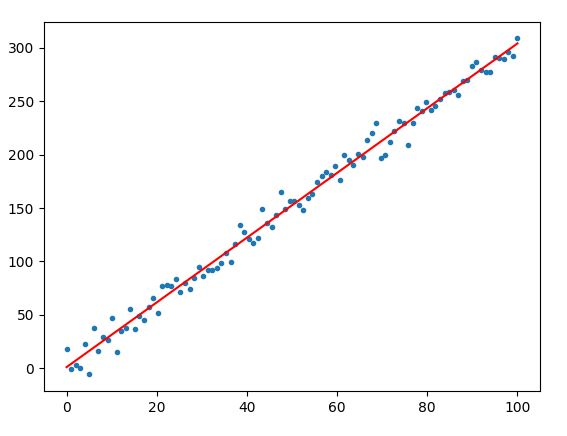
\includegraphics[width=0.75\textwidth]{figures/linefitdemoOutput}
\end{figure}

\end{frame}

%==============================================================

\begin{frame}[fragile]

\frametitle{Python code: line-fitting}

\vspace*{-3mm}

\texttt{linefitdemo.py}
\vspace*{-2mm}
\begin{lstlisting}[style=CStyle,basicstyle=\scriptsize]
# linefitdemo
import numpy as np
from scipy.optimize import curve_fit
import matplotlib.pyplot as plt

def line(x, m, b):
    return m * x + b

np.random.seed(1)   # replicate results by fixing seed
x = np.linspace(0, 100, 100)
y = 3. * x + 2. + np.random.normal(0., 10., 100)
plt.plot(x, y, '.')

popt, pcov = curve_fit(line, x, y)
m = popt[0]
b = popt[1]
print('Straight-line gradient m = {:.2f}'.format(m))
print('Straight-line intercept b = {:.2f}'.format(b))

xfine = np.linspace(0., 100., 100)
plt.plot(xfine, line(xfine, m, b), 'r')
plt.show()
\end{lstlisting}

\end{frame}

%==============================================================

\begin{frame}[fragile]

\frametitle{Python code: commentary}

\begin{itemize}
	\item lines 6--7: prepare to fit a straight line to $(x,y)$ data
	\begin{itemize}
		\item line equation $y = mx + b$
	\end{itemize}
	\item[]
	\item lines 9--12: create and plot $(x,y)$ data pairs
	\begin{itemize}
		\item straight line (gradient $3$ and $y$-intercept $b$)
		\item[] + Gaussian noise ($\mu=0, \sigma=10$)
	\end{itemize}
	\item[]
	\item lines 14--16: where the action happens!
	\begin{itemize}
		\item \texttt{curve\_fit()} function calculates $m$ and $b$ which provide best fit to $(x,y)$ data
	\end{itemize}
	\item[]
	\item lines 20--21: plot best-fit straight line
\end{itemize}

\end{frame}

%==============================================================

\begin{frame}[fragile]

\frametitle{Application of line-fitting: sea-ice extent}

\vspace*{-5mm}

\begin{figure}[ht]
	\centering
	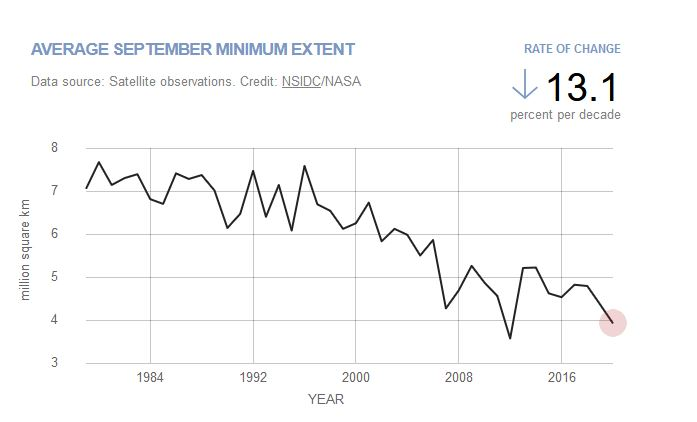
\includegraphics[width=.9\textwidth]{figures/seaiceextent}
\end{figure}

\href{https://climate.nasa.gov/vital-signs/arctic-sea-ice/}{https://climate.nasa.gov/vital-signs/arctic-sea-ice/}

\end{frame}

%==============================================================

\begin{frame}[fragile]

\frametitle{Fitting a straight line to sea-ice data}

\begin{itemize}
	\item graph shows average monthly Arctic sea ice extent each September since 1979, derived from satellite observations
	\item[]
	\item[] \textbf{Aim:} use straight-line fit to data to estimate when Arctic will be free of sea-ice
	\begin{itemize}
		\item ie: when sea-ice extent is zero
	\end{itemize}
	\item[]
	\item Key steps in solution
	\begin{enumerate}
		\item fit straight line to data, using \texttt{scipy.optimize.curve\_fit}
		\item line $y = mx + b$ intersects $x$-axis ($y=0$) when $x = -b/m$
	\end{enumerate}
\end{itemize}

\end{frame}

%==============================================================

\begin{frame}[fragile]

\frametitle{Python code: sea-ice extent}

\vspace*{-3mm}

\texttt{seaice.py}
\begin{lstlisting}[style=CStyle,basicstyle=\scriptsize]
# seaiceextent
import numpy as np
import matplotlib.pyplot as plt
from scipy.optimize import curve_fit

def line(x, m, b):
    return m * x + b

# dataset: September sea-ice extent 1979-2020
# https://climate.nasa.gov/vital-signs/arctic-sea-ice/
year = np.arange(1979, 2021)
extent = np.array([7.05,7.67,7.14,7.3,7.39,6.81,6.7,7.41,
        7.28,7.37,7.01,6.14, 6.47,7.47,6.4,7.14,6.08,
        7.58,6.69,6.54,6.12,6.25,6.73,5.83,6.12,
        5.98,5.5,5.86,4.27,4.69,5.26,4.87,4.56,
        3.57,5.21,5.22,4.62,4.53,4.82,4.79,4.36,3.92])
\end{lstlisting}

\begin{itemize}
	\item lines 6--7: prepare to fit a straight line to data
	\item lines 11--12: sea-ice extent dataset, 1979--2020
\end{itemize}

\end{frame}

%==============================================================

\begin{frame}[fragile]

\frametitle{Python code: sea-ice extent}

\vspace*{-3mm}

\texttt{seaice.py}---continued
\vspace*{-1mm}
\begin{lstlisting}[style=CStyle,basicstyle=\scriptsize]
popt, pcov = curve_fit(line, year, extent)
m = popt[0]         # gradient of best straight-line fit
b = popt[1]         # intercept

yearto2080 = np.arange(1979,2080)

print('extent(yr) = {:.3f}*year + {:.3f}'.format(m, b))
print('Estimate September sea-ice extent is 0 in year = {}'.format(int(-b/m)))
plt.plot(year, extent, 'o')
plt.plot(yearto2080, line(yearto2080, m, b), 'r')
plt.plot(-b/m,0,'gs')   # green square when ice extent is zero
plt.xlabel('Year')
plt.ylabel('September sea-ice extent (million sq km)')
plt.grid()
plt.show()
\end{lstlisting}
\vspace*{-2mm}
\begin{itemize}
	\item lines 1--3: fit line to data: $x=$~year, $y=$~extent
	\item line 5: straight line fit over years 1979--2080
	\item line 8: line intersects horizontal axis at $-b/m$
\end{itemize}

\end{frame}

%==============================================================

\begin{frame}[fragile]

\frametitle{Estimate Arctic sea-ice free in year 2071}

\begin{figure}[ht]
	\centering
	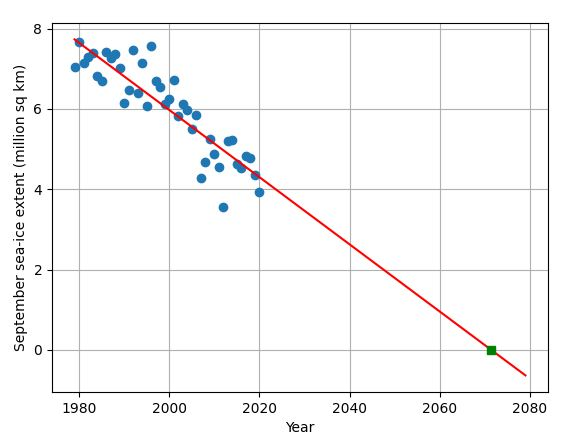
\includegraphics[width=.8\textwidth]{figures/seaiceextentOutput}
\end{figure}

\end{frame}

%==============================================================

\begin{frame}[fragile]

\frametitle{Lecture summary}
\begin{itemize}
	\item Normal distribution
	\item[]
	
	\item Fitting straight line to data
	\item[]
	
\end{itemize}

\end{frame}

\end{document}